\documentclass{article}

\usepackage[utf8]{inputenc}
\usepackage[english]{babel}
\usepackage{mathrsfs,amsmath}
\usepackage{float}
\usepackage{subfig}
\usepackage{units}
\usepackage{cite}
\usepackage{slashbox}
\usepackage{subfiles}
\usepackage{listings}
\usepackage{color}

\usepackage[a4paper]{geometry}	% enlarges the page margins to standard A4 paper
\usepackage{fancyhdr}		          % header usepackage
\usepackage{graphicx}		         % figures usepackage
\usepackage{mathtools}                       % Used in some equations for displaying text
\usepackage{amsmath}                        % No idea what it is, but seems usefull
\usepackage{amssymb} 		        % symbol for set
\usepackage{mathrsfs}                        %lagrange symbol
\usepackage{float}
\usepackage{epstopdf}

% Puts captions of tables on top
\floatstyle{plaintop}
\restylefloat{table}

% Puts captions in bold
\captionsetup{labelfont=bf}

\usepackage[ampersand]{easylist}


\begin{document}

\begin{titlepage}
  \begin{center}
%   \hr \\[1em]
   { \Huge Control for High Resolution Imaging} \\ 
   { \Large Adaptive Optics in Python - Wavefront Generation} \\   
%   \hr   
   \vfill
   \today \\[1em]
   
   \begin{tabular}{c}
    Lars Sybren van Leeuwaarden\\
   \end{tabular}\\
  \end{center}
 \end{titlepage}
 
\tableofcontents

\newpage

\section{Introduction}
\subsection{Overview on Wavefront Generation}
The goal of the wavefront generation part of the project Adaptive Optics in Python is as the name suggests, to create a wavefront that can be processed by the following sections of the adaptive optics. For the current implementation of the wavefront generation, the wavefront generation is split into two sections. The first one is the creation of aberrations in the optical set-up deterministic Zernike modes. The second part involves the creation of aberrations based on stochastic analysis of atmospheric aberrations. 

The distinction between these two sections is somewhat ambiguous, as both of these components will be added up to combine to the final wavefront. The choice to separate them is more based on implementation considerations rather then mathematical reasons. 

The current implementation of the wavefront generation is static. There is no temporal dependency implemented. This can be a shortcoming in phase screen generation, as it currently cannot model a passing cloud for example. The choice for this is simply because project was bounded. This is a topic for improvement in the future. Where possible, effort has been done to make the wavefront generation code ready to be extended in the future. Simply by adding functions and methods to the classes and making existing functions and methods easy to be extended - the object oriented programming approach. 

\subsection{Wave Equation}
The behaviour of light is, as is well known, explained by Maxwell's equations. Clever substitution of Amp\`{e}re's law into Faraday's law - or vice versa - and using Gauss' law to ensure dependency on only the magnetic field or the electric field. This will yield a neat equation where the wave behaviour is naturally apparent, the wave equation. This reader is probably not the best location to bore you with the entire derivation of the wave equation. It is however important to remember the plane wave behaviour of light later on, as it will make understanding much easier \footnote{For a more extensive derivation of the wave equation, please refer to the appendix.}.

In equation \ref{eq_wfg01}, the wave equation is given. In this equation, polarization is ignored. In the equation, $n^2 = \nicefrac{\epsilon}{\epsilon_0}$ is the ratio of the dielectric constants, or the refractive index and $c$ is the propagation speed of the wave, or the speed of light. The vector $U = (E, B)^T$ is the combined vector, containing the electric field and the magnetic field.

\begin{equation}
\label{eq_wfg01}
\left( \nabla^2 - \frac{n^2}{c^2} \frac{\partial^2}{\partial t^2} \right) U(\textbf{r},t) = 0 
\end{equation}

In order to solve equation \ref{eq_wfg01}, separation of variables is the usual approach. In this case, separating it in a spatially dependant part and a time dependant, hence $U(\textbf{r},t) = U(\textbf{r}) u(t)$. 

\begin{equation}
\label{eq_wfg02}
\left(\nabla^2 - \frac{\omega^2 n^2}{c^2}\right) U(\textbf{r}) = 0\\
\end{equation}
	
\begin{equation}
\label{eq_wfg03}
\left(\frac{\partial^2}{\partial t^2}- \frac{\omega^2}{n^2}\right) u(t) = 0
\end{equation}

\newpage
\section{Aberrations}
\subsection{Generalized Pupil Plane}
With the symmetry in time and propagation direction, solving the spatial derivative will suffice for a temporal analysis. This variant of the well known Helmholtz equation, will give the result in \ref{eq_wfg04}. Here the wavenumber $k_i = \nicefrac{2\pi}{\lambda_i}$ to separate the wave into it's respective spatial directions.

\begin{equation}
\label{eq_wfg04}
U(\textbf{r}) = A(x,y) e^{i n \textbf{k} \cdot \textbf{r} + \phi(x,y)}
\end{equation}

Equation \ref{eq_wfg04} can be simplified, for the goal of introducing the source of the aberrations. Here $\phi(x,y) = 2\pi W(x,y)$ is created a used in equation \ref{eq_wfg05}. Furthermore, the power function can be further separated in $z$-direction and $(x,y)$-directions. Hence: $P(z) = e^{i k z}$ and $P(x,y) = A(x,y) e^{i k p(x,y)}$, this makes sense if the $z$-direction is assumed to be the direction propagation. Since this is source of the radiation, $z$ can be set to zero, thus the exponent reduces to one. The result of these assumptions and simplifications introduce the generalized pupil function, $\mathcal{P}(x,y)$.

\begin{equation}
\label{eq_wfg05}
\mathcal{P}(x,y) = P(x,y) e^{i 2\pi W(x,y)}
\end{equation}

\subsection{Seidel Aberrations}
The pupil function $\mathcal{P}(x,y)$ introduces the wavefront $W(x,y)$. The wavefront introduces a phase offset on the wave which is not necessarily equivalent on the pupil plane. As such, it varies corresponding to the location $(x,y)$ on the plane. 
The wavefront $W$ could be any arbitrary number. However, commonly the wavefront is constructed of distinctive modes. Distinctive in the sense that the mode is linearly independent from the other modes, or in other words orthogonal.
This seems far fetched from this point, but consider optical set-ups where lenses can introduce for example a tilt, a defocus or a stigma to the image. These are distinctive or unique aberrations, from a physical point of view. That is, any one of the aberrations cannot be expressed in terms of the others.

\begin{table}[H]
\center
\begin{tabular}{c c}
Physical Description & Mathematical Expression\\
\hline \\
Piston Mode & $A_0$ \\
Lens tilt & $A_1 r \cos \theta + A_2 r \sin \theta$ \\
Defocus & $A_3 r^2$ \\
Stigma & $A_4 r^2 \cos(2\theta) + A_5 r^2 \sin(2\theta)$ \\
Coma & $A_6 r^3 \cos\theta + A_7 r^3 \sin\theta$ \\
Spherical Aberration & $A_8 r^4$
\end{tabular}
\caption{The first six physical modes of aberration, and their expression \cite{zernikeMatlabPag}.}
\label{tab_wfg01}
\end{table}

In table \ref{tab_wfg01}, a list of common aberrations is given together with a mathematical expression for the aberration. The parameters $A_i$ are the weights of the corresponding modes. The parameters $r$ and $\theta$ are the polar coordinates where $r$ is the normalized distance to the (local) optical origin, on the range $[0,1]$ and the angle $\theta$ defined the range $[0,2\pi]$.

Notice here how for example a defocus in the wavefront cannot be expressed in a linear multiple of a stigma or a lens tilt. In figure \ref{fig_wfg01} plots are given of the six distinctive aberrations described in the table.

\begin{figure}[H]
	\center
	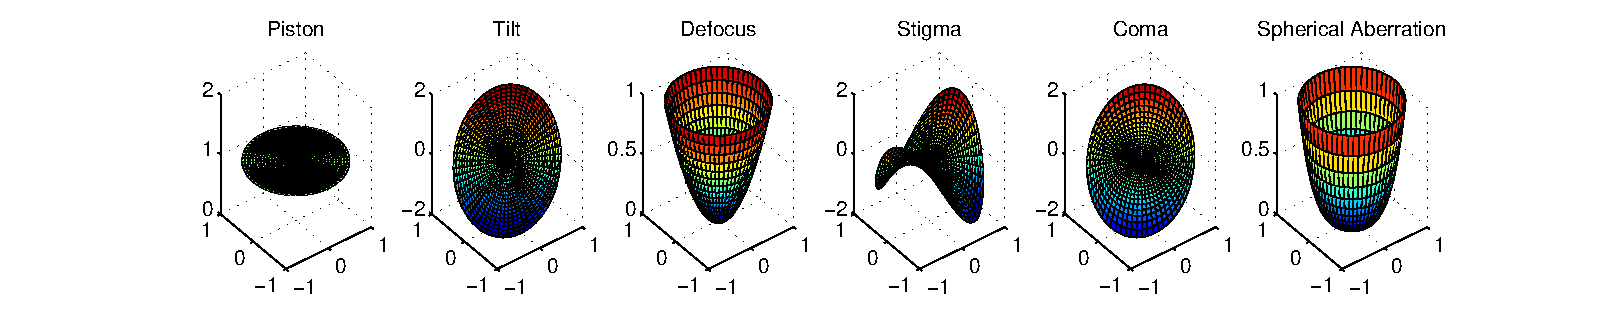
\includegraphics[width=1.05\textwidth, height=.2\textwidth]{Figures/Seibel.eps}
	\caption{Seibel aberrations.}
	\label{fig_wfg01}
\end{figure}

In order to create the total aberration of the wavefront, all the modes are summed together with their respective weights $A_i$. This will give polynomial series, the Seidel aberration, as is given in \ref{eq_wfg06}. In equation \ref{eq_wfg06} the polynomial expansion is limited to the stigma aberration.

\begin{equation}
\label{eq_wfg06}
W(x,y) = A_0 + A_1 r \cos \theta + A_2 r \sin \theta + A_3 r^2 + A_4 r^2 \cos(2\theta) + A_5 r^2 \sin(2\theta) + \dots
\end{equation}

This formula already gives a easy and reasonable representation of aberration. It however has limitations, which call for a better description of aberration, as will be pointed out in the section below, \ref{sec_wfgZer}.

\section{Zernike}
\label{sec_wfgZer}
Seibel aberrations are easy to compute, but have the downside of being limited in the mathematical sense. For the purpose of identifying weights of the various aberration modes, it is desired to have modes that are at least orthogonal to each other. This way decomposition in the different aberration modes is easy in later stages.

\subsection{Zernike Polynomials}
As with the Seibel aberrations, a polar coordinate system $[r,\theta]$ is used to express the location on the Zernike polynomial. This is a natural choice as most apertures are round. The polynomial is chosen such that the modes are orthogonal on the range $r \leq 1$ or $x^2 + y^2 \leq 1$. Further, the Zernike polynomals consist of a radial and an annular part with some scaling factor, like in equation \ref{eq_wfg07} \cite{zernikeCircle}.

\begin{equation}
Z^{m}_{n}(r,\theta) = A^{m}_{n} R^{m}_{n}(r) G^{m}_{n}(\theta)
\label{eq_wfg07}
\end{equation}

By definition, orthogonality of two possibly complex functions, can be found by taking the inner, or dot product of the two functions $V_i(x,y)$. With respect of the range of the function, it is possible to write the orthogonality as in equation \ref{eq_wfg08}.

\begin{equation}
\langle V_{\alpha}(x,y) , V_{\beta}(x,y) \rangle = \iint \limits_{x^2 + y^2 \leq 1} V_{\alpha}^{*}(x,y) V_{\beta}(x,y) dx dy = A_{\alpha,\beta} \delta_{\alpha,\beta}
\label{eq_wfg08}
\end{equation}

Now take $V_i(x,y) = V_i(r \cos \theta, r \sin \theta) = a_i r e^{\pm i m \theta} = R_i(r) G_i(\theta)$ and it can be proven that there is one and only one set of polynomials that is orthogonal in the interior of the unit circle. From the section on Seibel aberrations, it is clear that the total aberration is built from multiple modes. Thus validating the polynomial expansion from equations \ref{eq_wfg09} and \ref{eq_wfg10} \cite{zernikeCircle}, with the introduction of index $m$, indicating the angular mode. Furthermore, the index $n$ is introduced below to indicate the radial mode of the polynomial.

\begin{equation}
\mathcal{V}^{\pm m}_{n}(x,y)  = \mathcal{R}_{n} e^{\pm i m \theta}
\label{eq_wfg09}
\end{equation}

\begin{equation}
\mathcal{R}_{n}(r) = a^{m}_{k,0} r^{m} + a^{m}_{k,2} r^{m+2} +\dots+ a^{m}_{k,2k} r^{m+2k}
\label{eq_wfg10}
\end{equation}

The requirement of orthogonality modes can be put to use here. The orthogonality condition of equation \ref{eq_wfg08} can be expanded with the equations \ref{eq_wfg09} and \ref{eq_wfg10} above. Additionally, separating the orthogonality problem in the radial and angular part, as in equation \ref{eq_wfg11} and will allow to solve for a \textit{unique} set of orthogonal Zernike modes \cite{zernikeCircle}. 

\begin{equation}
\begin{cases}
\iint \limits_{x^2 + y^2 \leq 1} \mathcal{V}^{*m}_{n}(x,y) \mathcal{V}^{m}_{n}(x,y) dxdy &= a_n \delta_n  \\
\int \limits_0^1 \mathcal{R}^{*}_{n}(r) \mathcal{R}_{n}(r) r dr &= a_n \delta_n \\
\end{cases}
\label{eq_wfg11}
\end{equation}

Without getting to into the exact derivation, which is beyond the scope of this report, for that see \cite{zernikeCircle}. Equation \ref{eq_wfg11} guarantees orthogonality and completeness of the Zernike polynomials. In order to get a realization for the conditions specified, an orthogonalization is done. Note that $\mathcal{V}^{*m}_{n}(x,y)$ can be rewritten from polar to Cartesian format to a conditional sine-cosine relation as in equation \ref{eq_wfg12} \cite{zernikeMatlabPag}\cite{lectureNotes}\cite{zernikeCircle}.

\begin{equation}
\left.
\begin{matrix}
	V^{m}_{n}(x,y) & \\
	V^{*m}_{n}(x,y)
\end{matrix}
\right\rbrace =  R^{m}_{n}(r) e^{\pm i m \theta} =  R^{m}_{n}(r) 
\begin{cases}
	\sin(m\theta) &\text{odd mode}\\
	\cos(m\theta) &\text{even mode}
\end{cases}
\label{eq_wfg12}
\end{equation}

With the angular part of the equation solved, only the radial part is left. This is a somewhat less obvious derivation. Summarizing the Zernike polynomials, with respect to the format proposed in equation \ref{eq_wfg07}, equation \ref{eq_wfg13} is obtained \cite{zernikeMatlabPag}.

\begin{equation}
Z^{m}_{n}(r,\theta) = 
\begin{cases}
\sqrt{2(n+1)}R^{m}_{n}(r) G^{m}(\theta) & m \neq 0 \\
R^{0}_{n} & m = 0 
\end{cases}
\label{eq_wfg13}
\end{equation}

Where $R^{m}_{n}(r)$ is given by equation \ref{eq_wfg14}. Equation \ref{eq_wfg15} defines the angular part $G^m(\theta)$, similar to equation \ref{eq_wfg12}, just above. Note the the orthogonality framework presented here also sets limits on the choices of $n$ and $m$. Firstly, $|m| \leq n$, or even more precise $m = -n, -n+2,...,n-2,n$, see the exponent in equation \ref{eq_wfg10}. Secondly, $n \geq 0$ must also hold for the index $n$.

\begin{equation}
R^{m}_{n}(r) = \sum \limits^{(n-m)/2}_{s = 0}\frac{(-1)^s (n-s)!}{s! (\frac{n+m}{2}-s)! (\frac{n-m}{2}-s)!}r^{n-2s}
\label{eq_wfg14}
\end{equation}

\begin{equation}
G^m(\theta) = 
\begin{cases}
	\sin(m\theta) & m \text{ odd}\\
	\cos(m\theta) & m \text{ even}
\end{cases}
\label{eq_wfg15}
\end{equation}

\subsection{Noll Indices}
As explained in the section above, the indices $m$ and $n$ are bound to certain conditions set by the orthogonality constraint. Choosing some $n$ will give a range of possibilities for $m$. It is safe to say that this is not very practical and generally a mapping is chosen such that there is some integral number $i$ that maps to a specific $(m,n)$. The mapping $i \rightarrow (m,n)$ used here is the Noll mapping. Its system is given in table \ref{tab_wfg02} for the first 28 modes.

\begin{table}[H]
\center
\begin{tabular}{c | c c c c c c c c c c c c c c c}
\backslashbox{n}{m} &-6&-5&-4&-3&-2&-1&0&1&2&3&4&5&6 \\
\hline
0 & & & & & & &1& & & & & & \\
1 & & & & & &3& &2& & & & & \\
2 & & & & &5& &4& &6& & & & \\
3 & & & &9& &7& &8& &10& & & \\
4 & & &15& &13& &11& &12& &14& & \\ 
5 & &21& &19& &17& &16& &18& &20& \\
6 &27& &25& &23& &22& &24& &26& &28 \\
\end{tabular}
\caption{Noll's mapping of the first 28 modes. The number comprising the pyramid shape is the index $i$.}
\label{tab_wfg02}
\end{table}

When taking a closer look at the entries of the table, the values are not entirely arbitrary. It is obvious that negative values of $m$ have an odd index $i$ and positive values of $m$ have a even index. For the $m=0$, the odd and even indices are alternating, starting with a odd number at $n=0$.

Furthermore, the minimum index value at a any given row $n$ alternates at a set pattern: $m_n = 0,1,0,-1,0,1,0,-1,0,\dots$. This will make it easy to find starting point at for every radial mode $n$.

Now list the minima of the indices for every table row $n$: $i_{n}^{m=0} = [1,2,4,7,11,16,22,\dots]$. Then take take the difference of every element in the list: $\Delta i_{n}^{m=0} = [1,2,3,4,5,6,\dots]$. Indeed, every entry in the list $i_{n}^{m=0}$ is incremented with the next radial index $n$.
Thus, given some $i$ of the Noll index, it is possible to find the corresponding value $n$ by subtracting $\Delta i_{n}^{m=0} = [1,2,3,4,5,6,\dots]$ from $i$ one by one and checking if $i - \sum \Delta i_{n}^{m=0} \geq 0$.

The remainder can then be used to compute $m$.  By simply checking if $i$ is odd or even the, $m$ can be set positive or negative. For the actual value of $m$ take into account the alternating series of $m_n$ and the fact that they are defined on  range of $m$: $m = -n, -n+2,...,n-2,n$ as pointed out earlier.

This will give a single scalar that can be used to map to two scaler, making it much easier to compute wavefronts as will be pointed out in the next section. Figure \ref{fig_wfg06} plots the modes with corresponding Noll's index.

\newpage
\begin{figure}[H]
	\center
	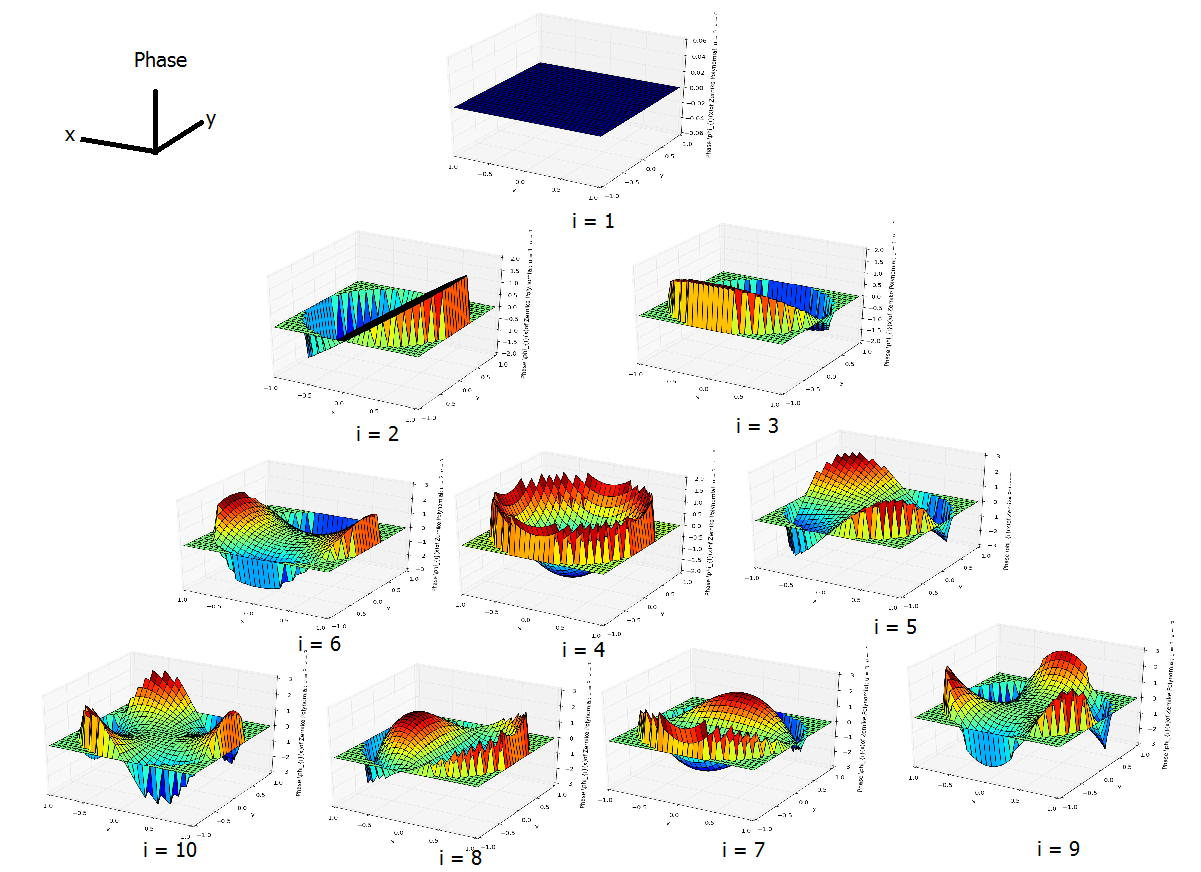
\includegraphics[width=1.0\textwidth, height=1\textwidth]{Figures/Nollsmap.png}
	\label{fig_wfg06}
	\caption{Noll's mapping, for the first then modes with corresponding plots of the Zernike modes in Python.}
\end{figure}


%%
%EXAMPLE IN PSEUDOCODE HERE? how to find (m,n) with i
%%

\newpage
\subsection{Constructing the Wavefront}
Remember the section on Seidel aberrations, a practical wavefront rarely exists of only one mode of aberration. Usually, it is a linear combination of multiple modes. With the guarantee of orthogonality between the various modes by definition, it easy to compose a sum for the linear combination, as in equation \ref{eq_wfg16} \cite{zernikeMatlabPag}. Also note how the newly introduced Noll indexing has replaced the former two indexes as in equation \ref{eq_wfg13}. Also note similarities with the field of dynamics. With dynamical systems, the time behaviour is a composition of the eigenmodes. The eigenvectors and eigenvalues determine the spatial direction and the natural frequency respectively. Since a static aberration is considered static for this coding project, only the spatial part is considered. Otherwise $W(r,\theta)$ can considered to be $W(r,\theta,t) = W(r,\theta)w(t)$, a similar decomposition a is considered in equations \ref{eq_wfg02} and \ref{eq_wfg03}.

\begin{equation}
W(r,\theta) = \sum \limits_{i=1}^{\infty} a_i Z_i(r,\theta)
\label{eq_wfg16}
\end{equation}

Equation \ref{eq_wfg16} introduces the weighting factor $a_i$. It has the same purpose as it had in the Seidel aberrations, to give a certain strength to a aberration mode. In figure \ref{fig_wfg02} a example is plotted. Here the weightings $a_i$ are defined as follows, corresponding to the following physical modes: tilt, defocus and a y-direction pentafoil respectively.

\begin{equation}
\begin{cases}
a_2 = 0.5 & i = 2 \\
a_4 = 0.25 & i = 4 \\
a_{21} = -0.6 & i = 21 \\
a_i = 0 & i \neq 2,4,21
\end{cases}
\label{eq_wfg17}
\end{equation}

\begin{figure}[H]
	\center
	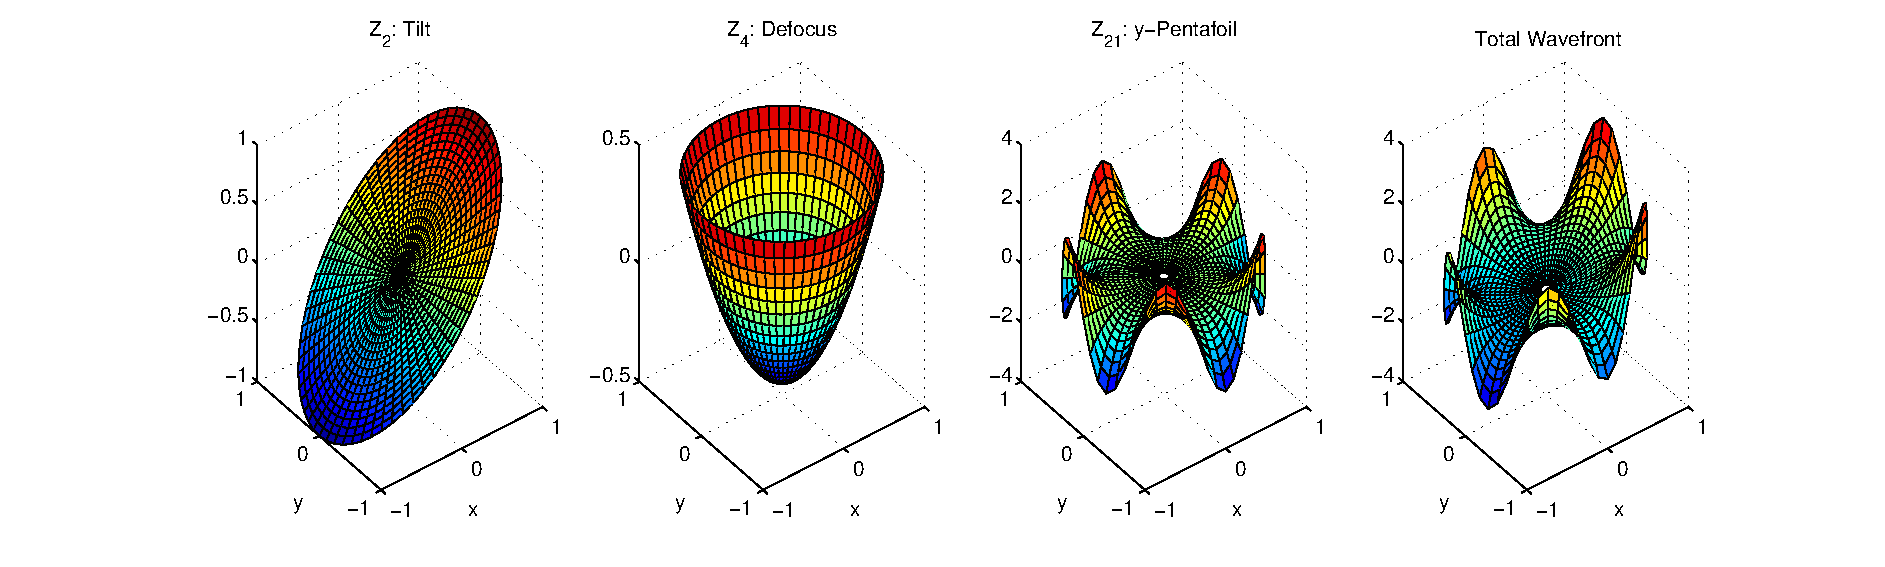
\includegraphics[width=1.0\textwidth, height=.3\textwidth]{Figures/Zernike.eps}
	\caption{Zernike aberrations. From left to right: tilt $Z_2$, defocus $Z_4$, y-pentafoil $Z_{21}$ and the composed wavefront $W(r,\theta)$.}
	\label{fig_wfg02}
\end{figure}

\newpage
\subsection{Decomposition of the Wavefront}
The framework built for constructing wavefront by adding the several desired modes, can also be used the other way round. Given some wavefront and a set of modes to be used, what weighting factors do the modes need to get in order to minimize the difference between the 'real' wavefront and the composed wavefront.

Again the definition of orthogonality for the Zernike comes in handy. That way the problem reduces to a decomposition of orthogonal projections, much like the well known Gram-Schimdt algorithm in linear algebra. It is not required to create a orthogonal basis, as the orthogonal bases comprises of the Zernike modes $Z_i$ where $W(r,\theta)$ needs to be projected on, which are already orthogonal.

Let's explain according to linear algebra concepts. Imagine two vectors $\textbf{a}$ and $\textbf{b}$. Now project vector $\textbf{a}$ onto the basis vector $\textbf{b}$, the amount of common mode of is given with the projection formula, see equation \ref{eq_wfg18} \cite{lay}.

\begin{equation}
\text{proj}_{\textbf{b}}(\textbf{a}) = \frac{\textbf{a} \cdot \textbf{b}}{\textbf{b} \cdot \textbf{b}} \textbf{b}
\label{eq_wfg18}
\end{equation}

In this case, it is not necessary to find the actual basis, that is already known. Thus the weighting is the only matter of interest, or the amount of common mode with respect to the basis vector $\textbf{b}$.  

From the crude Gram-Schimdt algorithm, it is possible to develop a algorithm which is more suited to the decomposition of the wavefront in a particular set of Zernike modes. Recall that only the amount of common mode, the weighting,  is desired as the basis is already orthogonal, see equation \ref{eq_wfg19}.

\begin{equation}
a_i =  \frac{\textbf{a} \cdot \textbf{b}}{\textbf{b} \cdot \textbf{b}}
\label{eq_wfg19}
\end{equation}
Rewriting the dot product into a the calculus format as in equation \ref{eq_wfg20}, as proposed earlier in equation \ref{eq_wfg08}.

\begin{equation}
a_i = \frac{\int \limits_{0}^{2\pi} \int \limits_{0}^{1} W(r,\theta) Z_i(r,\theta)}{\int \limits_{0}^{2\pi} \int \limits_{0}^{1} Z_{i}^{2}(r,\theta) }
\label{eq_wfg20}
\end{equation}

For a numerical implementation, it is necessary to discretize the system, as is done in equation \ref{eq_wfg21} \cite{zernikeMatlab}. Note the change in coordinate system, as the discrete grid is rectangular, for Fourrier transform purposes later on. Furthermore, $p$ and $q$ iterate over the grid formed by the discretization.

\begin{equation}
a_i = \frac{\sum \limits_p \sum \limits_q W(x_p,y_q) Z_i(x_p,y_q) }{\sum \limits_p \sum \limits_q Z_{i}^{2}(x_p,y_q) } 
\label{eq_wfg21}
\end{equation}

\newpage
Equation \ref{eq_wfg21} will satisfy, if only one mode requires computation. More often, it is desired to compute all modes simultaneously. On top of that, it is desired to utilize the numerical power of linear algebra.
For that, consider equation \ref{eq_wfg16}. Rewriting it results in equation \ref{eq_wfg22}.

\begin{equation}
W(x_p,y_q) = 
\begin{bmatrix}
Z_1 & | & Z_2 & | & \dots & | & Z_n
\end{bmatrix}
\begin{bmatrix}
a_1 \\
a_2 \\
\dots \\
a_n
\end{bmatrix}
\label{eq_wfg22}
\end{equation}

Rewriting $Z_i(x_p,y_q)$ to a vector in order to reduce the sets of systems to a single system of equations. Introduce $Z_i(x_p,y_q) = \bar{Z}_i(j)$ and $W(x_p,y_q) = \bar{W}(j)$, by stacking all the columns of $Z_i$ under each other. The system reduces to equation \ref{eq_wfg23}.

\begin{equation}
W(x_p,y_q) = \mathcal{Z}A = 
\begin{bmatrix}
\bar{Z}_1 & \bar{Z}_2 & \dots & \bar{Z}_n
\end{bmatrix}
\begin{bmatrix}
a_1 \\
a_2 \\
\dots \\
a_n
\end{bmatrix}
\label{eq_wfg23}
\end{equation}

Finding the vector of weights $A$ is easy now, by taking the pseudo-inverse as is done in equation \ref{eq_wfg24}. Note that the normal inverse generally does not work, as $\mathcal{Z}$ not square and not necessarily non-singular.

\begin{equation}
A = \left(\mathcal{Z}^T \mathcal{Z} \right)^{-1} \mathcal{Z}^T \bar{W}(j)
\label{eq_wfg24}
\end{equation}

However note here: $\mathcal{Z}$ is column orthogonal, hence it's construction in equation \ref{eq_wfg23}. If this is the case, $\mathcal{Z}^T \mathcal{Z}$ should reduce to a diagonal matrix \footnote{The matrix $\mathcal{Z}^T \mathcal{Z}$ is not identity, as equation \ref{eq_wfg08} allowed a scalar to exist in the orthogonality condition, the system is thus not orthonormal.}. 
Numerical inaccuracies in a computer will introduce derivations from true identity. More importantly, the wavefront is sampled with a finite number of samples. This can also cause the computation of $\mathcal{Z}^T \mathcal{Z}$ to no longer give "algebraic" diagonal matrices.

A small test was done with the code written for this project. For the small test, the modes and weights from equation \ref{eq_wfg17} were imputed to the code, together with a 30-by-30 grid. The relative difference between the diagonal entries and the upper and lower triangles of the matrix - excluding the diagonal entries - are in the order of $10^{16}$ and larger. Considering this, it is fair to state that the matrix is diagonal.

\newpage
\subsection{Validity of the Decomposition}
This method is in general only as good as the number of modes supplied to the decomposition. In general, more modes should give a better approximation of the real aberration. For validation purposes, it can be desired to compute the root mean square error - or standard deviation - that is introduced by using a finite series expansion of the Zernike modes. Equation \ref{eq_wfg25} \cite{zernikeMatlab} introduces  a algebraic framework for the RMS error for a 2D surface. In this equation $W(r,\theta)$ is the original wavefront and $\bar{W}$ the mean of the wavefront.

\begin{equation}
\sigma^2 = \frac{1}{\pi} \int \limits_0^{2 \pi} \int \limits_0^1 \left(W(r,\theta) - \bar{W} \right)^2 r dr d\theta
\label{eq_wfg25}
\end{equation}

With $\bar{W}$ behaving as a piston mode, thus as the mode $i = 1$ in Noll's indexing. It possible to introduce equation \ref{eq_wfg16} again into equation \ref{eq_wfg25}. In equation \ref{eq_wfg26} ], the last equation is substituted and split into a integral part and constant part.

\begin{equation}
\sigma^2 = \frac{1}{\pi} \sum \limits_{i=2}^{\infty} a_i \sum \limits_{i=2}^{\infty} a_i' \int \limits_0^{2 \pi} \int \limits_0^1 Z_i(r,\theta) Z_i'(r,\theta) r dr d\theta
\label{eq_wfg26}
\end{equation}

Then recall the orthogonality property from \ref{eq_wfg08} and computing $\pi$ as the constant for the Zernike orthogonality, then equation \ref{eq_wfg27} is obtained.

\begin{equation}
\sigma^2 = \frac{1}{\pi} \sum \limits_{i=2}^{\infty} a_i \sum \limits_{i=2}^{\infty} a_i' \pi \delta_{ii'}
\label{eq_wfg27}
\end{equation}

Reducing to equation \ref{eq_wfg28}, due to the Dirac delta function. Also consider it with substitution of the result of equation \ref{eq_wfg24}.
\begin{equation}
\sigma^2 = \sum \limits_{i=2}^{\infty} a_i^2 = A^T A
\label{eq_wfg28}
\end{equation}

A powerful result, as the variance on the wavefront is simply the sum weights squared. Again by made easy by the orthogonal properties of the Zernike modes.

\newpage
\section{Atmospheric Aberrations}
\subsection{Turbulence in the Atmosphere}
If you've ever looked up to the night's clear sky and looked at a star, you've probably noticed a twinkling. Now, the visual surface of a star is by far a steady surface, so the twinkles might be down to intensity variations. But considering the huge distance between Earth and the star, it is not possible to distinguish these variations with our eyes. Instead, this 'twinkling' down to column of atmosphere that between the star and the eye. The air in the atmosphere is obviously not a vacuum and thus has a refractive index. 

This refractive index is close to unity compared to the vacuum. Usually close enough to pretend as if the light was travelling trough a vacuum. However, as distance through the medium increases and as the medium is showing turbulence, it becomes a problem for the static optical set-up. From equation \ref{eq_wfg01} it can be shown that changes in the refractive index will directly influence the frequency of the light wave. Thus changes in refractive index, combined with continuity of electromagnetic fields and conservation of energy, will cause changes in propagation speed of the wave and hence changes in the direction of propagation of the wave. This in turn will be observed as phase shifts to the observer.

Thus the model to introduce will need to describe variations in the refractive index in the path of a light wave. The variations in refractive index, caused by temperature differences, pressure differences and air humidity. This creates equations like the Edlen equation \cite{edlen1966}. Empirical equations and often upgraded and amended to fit new measurements. 

Unfortunately, none of the parameters, like the temperature at any height, are available for observers on the ground. This will complicate the use of (modified \footnote{The term 'modified' is used in the sense that it uses the common Fresnel propagation of light in vacuum and exploits the fact that the refractive index is close to one.}) Fresnel propagation theory for example, the Split-Step Beam Propagation Method. Therefore, statistical models are introduced that match the statistic properties of a column of air.

\subsection{Kolmogorov}
Simply by the fact that an algebraic model is extremely difficult to come by with this many parameters. It will involve creating solutions for the Navier-Stokes equation, a non-linear problem for developed turbulent flows.
The Kolmogorov theory of turbulence introduced the idea of matching statistical behaviour of a model with that of experimental data, based on turbulent flows \cite{kolmogorov1941local}. 

From fluid dynamics, the average size of turbulence 'bubbles' or eddies, can be related to their speed via the proportionality in equation \ref{eq_wfg29}. Note thet for the functions to come isotropy and local homogeneity  is assumed. That is, fully developed turbulence is assumed and spatial changes in the turbulences are 'quasi-static'.

\begin{equation}
v \propto r^{\frac{1}{3}}
\label{eq_wfg29}
\end{equation}

\newpage
From this point a structure function is used $D(r) = c^2 v^2$. The structure function is created from the statistical properties of the aberrations.  In the structure function here, the constant $c$ is dependant on the length scale, as is given in the equation set \ref{eq_wfg30}. Here two length scales are introduced, the inner small scale and the largest scale. The inner scale $l_0$ is in the range of the smallest turbulence bubble. $L_0$ on the other hand is in the range of the height of the atmosphere column \cite{zernikeMatlab}.

\begin{equation}
D_v(r) = 
\begin{cases}
C_v^2 l_0^{-\frac{4}{3}} r^{\frac{2}{3}} & 0 \leq r \ll l_0\\
C_v^2 r^{\frac{2}{3}} & l_0 \ll r \ll L_0 
\end{cases}
\label{eq_wfg30}
\end{equation}

Similarly, this can be done for the relation between $r$ and the temperature potential $\theta$, this proportionality reads $r \propto \theta^{\frac{1}{3}}$. Again creating the structure functions as in set \ref{eq_wfg31} \cite{zernikeMatlab}.

\begin{equation}
D_\theta(r) = 
\begin{cases}
C_\theta^2 l_0^{-\frac{4}{3}} r^{\frac{2}{3}} & 0 \leq r \ll l_0\\
C_\theta^2 r^{\frac{2}{3}} & l_0 \ll r \ll L_0 
\end{cases}
\label{eq_wfg31}
\end{equation}

Now for the index of refraction $n$ is made as a stochastic variable and is introduced as in equation \ref{eq_wfg32}. Note that the expected value of the refractive index is close to one as this is a property of air and the stochastic variable $n_1$ can be empirically found as in equation \ref{eq_wfg33}. Here $P(r)$ represents the pressure, $T(r)$ the ordinary temperature and $\lambda$ the wavelength \cite{zernikeMatlab}.

\begin{equation}
n(r) = \mu_n + n_1(r)
\label{eq_wfg32}
\end{equation}

\begin{equation}
n_1(r) = 77.6 \cdot 10^{-6} (1 + 7.52 \cdot 10^{-3} \lambda^2) \frac{P(r)}{T(r)}
\label{eq_wfg33}
\end{equation}

Taking the derivative of the refractive index, and assuming the wavelength equal to $\lambda  = 500 \text{nm}$, equation \ref{eq_wfg34} is obtained \cite{zernikeMatlab}.

\begin{equation}
dn = 7.99 \cdot 10^{-5} \left( dP - \frac{-dT}{T^2} \right)
\label{eq_wfg34}
\end{equation}

Now assume the pressure locally constant in the turbulence bubble, and the temperature relation to the temperature potential as $d\theta = d(T - T_0) = dT$. Thus assuming the reference temperature $T_0$ constant in the bubble.  This allows to reduce the change in refractive index to equation \ref{eq_wfg35}.

\begin{equation}
dn = 7.99 \cdot 10^{-5} \frac{d\theta}{T^2}
\label{eq_wfg35}
\end{equation}

Recall equation \ref{eq_wfg31} and observe that the derivative of the  refractive index is proportional to the derivative of the potential temperature. Thus the structure function of the potential temperature can be used to describe the structure function of the refractive index, under the assumptions described above as in equation \ref{eq_wfg36} \cite{zernikeMatlab}.

\begin{equation}
D_n(r) = 
\begin{cases}
\left[7.76 \cdot 10^{-7} \left(1 + 7.52 \cdot 10^{-3} \lambda^{-2} \right) \frac{P}{T^2} \right]^2 C_\theta^2 l_0^{-\frac{4}{3}} r^{\frac{2}{3}} & 0 \leq r \ll l_0\\
\left[7.76 \cdot 10^{-7} \left(1 + 7.52 \cdot 10^{-3} \lambda^{-2} \right) \frac{P}{T^2} \right]^2 C_\theta^2 r^{\frac{2}{3}} & l_0 \ll r \ll L_0 
\end{cases}
\label{eq_wfg36}
\end{equation}

Using the structure function found above for the index of refraction, it is now possible to calculate a power spectral density of the refractive index. Power spectral density allows transforms the structure functions to their corresponding spatial frequency domain \cite{zernikeMatlab}.

\begin{equation}
\Phi_n(f) = \frac{1}{4 \pi^2 f^2} \int \limits_0^\infty \frac{\sin(f r)}{f r} \frac{d}{dr} \left[ r^2 \frac{d}{dr} D_n(r) \right] dr
\label{eq_wfg37}
\end{equation}

Here the spatial frequency $f$ is defined as $f = 2 \pi (f_x + f_y)$ The spatial frequency components in $x$ and $y$ direction of the phase plane. The integral computes to equation \ref{eq_wfg38}, the Kolmogorov power spectral density function. The spatial frequency term is introduced here as $f^2 =f_x^2 + f_y^2$ \cite{zernikeMatlab} \cite{lectureNotes} \footnote{In the original article proposed by A.N. Kolmogorov in 1939, he actually proposed a proportionality to a length $r$ \cite{kolmogorov1941local}, rather then equalities. Only later sources such as \cite{zernikeMatlab} describe an actual scalar.}.. 

\begin{equation}
\begin{matrix}
\Phi_n(f) = 0.033 C_n^2 f^{\frac{-11}{3}} & \text{for} & \frac{1}{L_0} \leq f \leq \frac{1}{l_0}
\end{matrix}
\label{eq_wfg38}
\end{equation}

What remains, is the term $C_n$ to be computed. Using the result from equation \ref{eq_wfg05}, it is possible to derive a mean value for the optical field, as in equation \ref{eq_wfg39} and the covariance of the optical field in equation \ref{eq_wfg40}, both calculated from Rytov theory.

\begin{equation}
\langle U(\textbf{r}) \rangle = U_0(\textbf{r})\langle e^{\psi(\textbf{r})} \rangle
\label{eq_wfg39}
\end{equation}

\begin{equation}
B(\textbf{r},\textbf{r}^{'}) = \langle U(\textbf{r}) U^{*}(\textbf{r}^{'}) = e^{-\frac{1}{2} D_\phi(\textbf{r})}
\label{eq_wfg40}
\end{equation}

The covariance function can be used to compute the coherence factor of the wave given in equation \ref{eq_wfg41}. Also note that the spatial position on the wavefront $\textbf{r}$ can be replaced by a distance between the points $\textbf{r}$ and $\textbf{r}^{'}$ as the the system is assumed isotropic and homogeneous \footnote{In other words the travelled path of the light is assumed not to be of interest, in is considered not to be a path integral. As if the distortions are 'white', to see it's time domain equivalence. }. 

\begin{equation}
\mu(\textbf{r},\textbf{r}^{'},z) = \frac{B(\textbf{r},\textbf{r}^{'},z) B(\textbf{r},\textbf{r}^{'},z)}{B(\textbf{r},\textbf{r},z) B(\textbf{r}^{'},\textbf{r}^{'},z)} = \mu(|\Delta \textbf{r}|,z)
\label{eq_wfg41}
\end{equation}

Using the same principle of the structure functions as was done previously with the refraction index, temperature and turbulence bubble speed, a structure function for the wavefront is introduced as in equation \ref{eq_wfg42}. Under the assumption that it behaves as plane wave \cite{lectureNotes}.

\begin{equation}
D(\textbf{r},\textbf{r}^{'}) = -2 \ln \mu(\textbf{r},\textbf{r}^{'}) =  D_\chi(\textbf{r},\textbf{r}^{'}) + D_\phi(\textbf{r},\textbf{r}^{'})
\label{eq_wfg42}
\end{equation}

The last equation combined with the PSD function from equation \ref{eq_wfg37}, but only with $D_n$ and $\Phi_n$ replaced by $D_\phi$ and $\Phi_\phi$ respectively. Without going into the extensive derivation \cite{sasiela2007electromagnetic}: the results for $\mu$ are obtained in equation \ref{eq_wfg43} for a plane wave \cite{zernikeCircle}.

\begin{equation}
\mu(|\Delta \textbf{r}|,z) = \exp \left\{ -4 \pi^2 k^2 \int \limits_0^{\Delta z} \int \limits_0^\infty \Phi_n(f,z)(1 - J_0(f |\Delta \textbf{r}|)) df dz \right\}
\label{eq_wfg43}
\end{equation}

The actual evaluation of $\mu$ will depend on the assumptions taken. Since Kolmogorov is the reference frame for now, the spatial frequency $f$ is limited to the range $ \frac{1}{L_0} \leq f \leq \frac{1}{l_0}$. Now $C_n$ will need to be replaced by quantities from experimental data, the quantity $\mu$.

As such, $\mu$ can be expressed as in equation \ref{eq_wfg44} under Kolmogorov assumptions. The constant constant is determined in from the Strehl ratio for various aperture diameters \cite{tubbs2003lucky}.

\begin{equation}
\mu^{Kol}(|\Delta \textbf{r}|,z) = \exp \left\{ -1.46 k^2 |\Delta \textbf{r}|^{\frac{5}{3}} \int \limits_0^{\Delta z} C_n^2(z) dz \right\}
\label{eq_wfg44}
\end{equation}

\newpage
Now, introducing the Fried parameter $r_0$, the typical scale length of the turbulence, as is done for a plane wave in equation \ref{eq_wfg45}\cite{lectureNotes} \cite{zernikeCircle}.

\begin{equation}
r_0 = 0.423 k^2 |r_0|^{\frac{5}{3}} \int \limits_{0}^{\Delta z} c_{n}^2(h) dz
\label{eq_wfg45}
\end{equation}

Also $D_\phi$ in equation \ref{eq_wfg46} and $B(\Delta \textbf{r})$ in equation \ref{eq_wfg47} can be obtained and expressed in the Fried parameter \cite{zernikeCircle}.

\begin{equation}
D_\phi(\textbf{r},\textbf{r}^{'}) = 6.88 \left(\frac{|\textbf{r}|}{r_0}\right)^{\frac{5}{3}}
\label{eq_wfg46}
\end{equation}

\begin{equation}
B(\textbf{r}) = e^{-3.44 \left(\frac{|\textbf{r}|}{r_0} \right)^{\frac{5}{3}}}
\label{eq_wfg47}
\end{equation}

All things considered, $C_n$ can now be replaced from the Kolmogorv PSD equation as suggested in \ref{eq_wfg48}. Here $C_n$ is replaced with the Fried parameter, the characteristic scale length of the turbulence.

\begin{equation}
\begin{matrix}
\Phi_n(f) = 0.023 r_0^{-\frac{5}{3}} f^{\frac{-11}{3}} & \text{for} & \frac{1}{L_0} \leq f \leq \frac{1}{l_0}
\end{matrix}
\label{eq_wfg48}
\end{equation}

\newpage
\subsection{Power Spectral Densities}
As indicated in equations the validity of the Kolmogorov power spectral density is limited to a range of $\frac{1}{L_0} \leq f \leq \frac{1}{l_0}$. These bounds can be limiting in some cases. The solution is partly in evaluating the equation in the paragraphs above again, but now with other constraints set on the spatial frequency.

A other PSD for practical implementation is the von K{\'a}rm{\'a}n PSD and the modified von K{\'a}rm{\'a}n. Their respective PSD's are given in the equations below in equation \ref{eq_wfg49} and \ref{eq_wfg50} \cite{zernikeCircle}. Note the strong similarities between the PSD, only element are added that become increasingly dominant on certain ranges of spatial frequency.

\begin{equation}
\begin{matrix}
\Phi_n^{vKar}(f) = \frac{0.023 r_0^{\frac{5}{3}}}{\left(f^{2} + f_{0}^{2}\right)^{\frac{11}{6}}} & \text{for} & 0 \leq f \leq \frac{1}{l_0}
\end{matrix}
\label{eq_wfg49}
\end{equation}

\begin{equation}
\begin{matrix}
\Phi_n^{MvKar}(f) = \frac{0.023 r_0^{-\frac{5}{3}} \exp\left\{\frac{f^2}{f_m^2}\right\} } {(f^2 + f_0^2)^{\frac{11}{6}}}  & \text{for} & 0 \leq f < \infty
\end{matrix} 
\label{eq_wfg50}
\end{equation}

Von K{\'a}rm{\'a}n removes the lower boundary and modified Von K{\'a}rm{\'a}n also removes the upper boundary. Other PSD, like Tararskii, remove the upper boumd compared to Kolmogorov PSD. in figure \ref{fig_wfg03}, Kolmogorov and Von K{\'a}rm{\'a}n power spectral densities are plotted. The way it is presented shows strong similarities with bode plots. The spatial frequency is then replaced by time frequency, but still the $y$-axis can be considered a gain at a certain frequency.
 
\begin{figure}[H]
	\center
	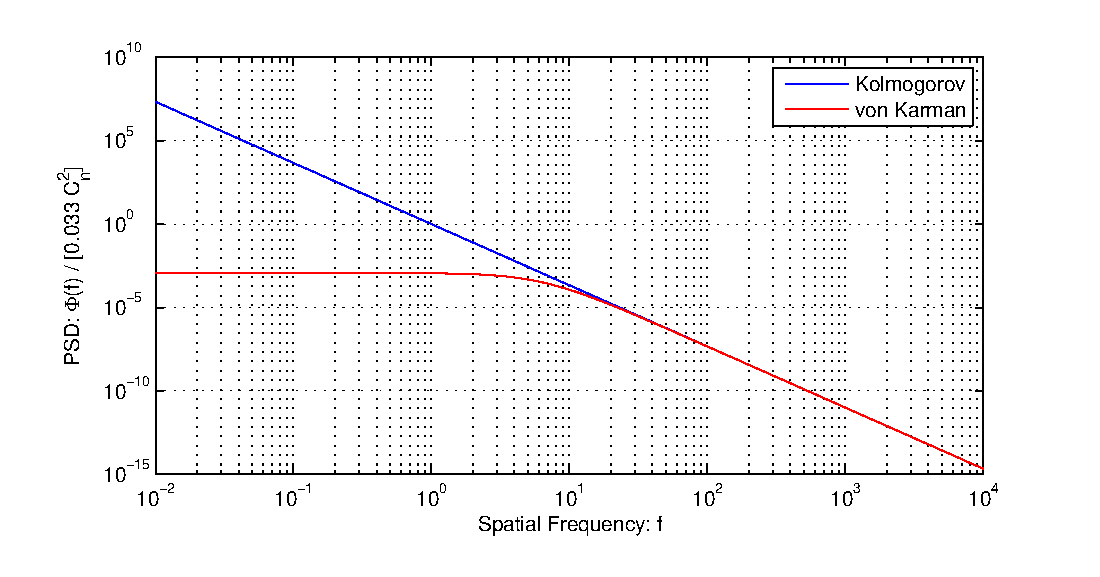
\includegraphics[height=1.0\textwidth, height=.3\textwidth]{Figures/kolmogorov.eps}
	\caption{Kolmogorov and von K{\'a}rm{\'a}n power spectral density functions, $L_0$ set to one, normalized in the common constant of both PSD functions.}
	\label{fig_wfg03}
\end{figure}

\newpage
\subsection{Discrete Phase Screens}
So far the phase screen was considered to be continues of nature. Both in the plane of the phase, but also in the direction of propagation. Let's first consider discretization the direction of propagation. Consider the light wave to be travelling through a series of Phase Screen that distort the phase of the incoming wavefront. Equation \ref{eq_wfg51} \cite{zernikeCircle} introduces the series of phase screens. Consider it to have have different independent stages of travelling of the wave trough different aberrations.

\begin{equation}
\sum \limits_{i=0}^{n} C_n^2 z_i^m \Delta z_i
\label{eq_wfg51}
\end{equation}

Now the phase plane will need to be dicretized as well for an implementation in code. Consider the Fourier  of the phase screen in discrete form in equation \ref{eq_wfg52}.

\begin{equation}
\phi(x,y) = \sum \limits_{n = -\infty}^{\infty} \sum \limits_{m = -\infty}^{\infty} c_{m,n} e^{2 \pi j (f_{xn} x + f_{ym} y)}
\label{eq_wfg52}
\end{equation}

The term $c_{m,n}$ represents the Fourier weights. As the atmosphere was modelled as stochastic process, these weights will need to satisfy statistics of the atmosphere. For that the realization of the Fourier coefficients is drawn from a normal or Gaussian distribution. The draws are spatially independent from each other. Similar how white noise in time domain is drawn independent with respect to other time instance but itself. Since $c_{m,n}$ is in general a complex constant, both the real and complex part will need to be drawn from a normal distribution. In equation \ref{eq_wfg53} a random phase screen is a every spatial frequency point $f$. It is then weighted with the PSD simply by multiplication. This feature can be exploited as the numbers are drawn from the normal distribution $N(0,1)$ in Fourier domain, rather then doing a convolution. 

\begin{equation}
\mathcal{F}\{ \phi(x,y)\} =  \left( N(0,1) + i N(0,1) \right)(f) \sqrt{\Phi_{\phi}(\textbf{r})} \Delta f 
\label{eq_wfg53}
\end{equation}

The transformation back to the real spatial domain can be done efficiently by a Fast Fourier Transform. However practical problems arise when this method is used in a coding environment. Since every sample is taken at complete random in Fourier domain, discrepancies arise in low spatial frequency due to spectral leakage \cite{lane1992simulation}. Using the equation of the phase structure function of equation \ref{eq_wfg46}: in low frequency, that is in high $\frac{| \Delta \textbf{r}}{r_0}|$, it will be lower in simulation with respect to the theory proposed in high frequency.

Many solutions have been proposed to make up for the error arising in the low frequency domain. Some have tried to introduce random draws from Zernike modes as a compensation. This will obviously run into trouble when decomposing in the wavefront in Zernike modes, as one will find the "random" mode directly back during decompression. An alternative method is the "subharmonics" method \cite{zernikeCircle}. %pages 168-169

The subharmonics method used in the implementation was introduced by Lane \textit{et al.}  \cite{lane1992simulation}. It divides a grid point in the spatial frequency domain in consecutively smaller and smaller 3-by-3 grids, like the example of \ref{fig_wfg04}

\newpage
\begin{figure}[H]
	\center
	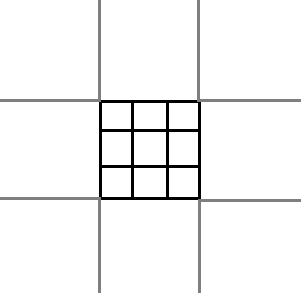
\includegraphics[height=.5\textwidth, height=.3\textwidth]{Figures/subharmonics.png}
	\caption{The subharmonics division grid, here only 2 divisions are shown.}
	\label{fig_wfg04}
\end{figure}

For every subdivision, the same method is repeated as was outlined in equation \ref{eq_wfg53}. In order to make sure that the power of the signal in all the subdivisions remains in the statics set the the aberration, weights are introduced. The weights are easy to compute, as they must be equal to the area in spatial domain covered. The final phase screen is simply the addition of all the subdivision and the "high frequency" phase screen from equation \ref{eq_wfg53}. Equation \ref{eq_wfg54} proposes the used format.

\begin{equation}
\mathcal{F}\{\phi(x,y)\} = \sum \limits_{p=1}^{N_p} \sum \limits_{f_x=-\infty}^\infty \sum \limits_{f_y=-\infty}^\infty c_p \left( N(0,1) + i N(0,1) \right)(f_{x,p},f_{y,p}) \sqrt{\Phi_{\phi}(\textbf{r})} \Delta f_p
\label{eq_wfg54}
\end{equation}

For practical reasons, $p$, $f_x$ and $f_y$ are finite. In the code $p$ is limited to three and the sample grid is picked by the user. Note that there is no reason to take lower frequencies into account then the sample length of the data set. On the other side, there is no reason to take into account frequencies above the Nyquist criterion. Furthermore, the choice of $r_0$, for von K{\'a}rm{\'a}n also $l_0$ and $L_0$, must be outside of the sample length and Nyquist constraints. In figure \ref{fig_wfg05} a realization of a Kolmogorov phase aberration.

\begin{figure}[H]
	\center
	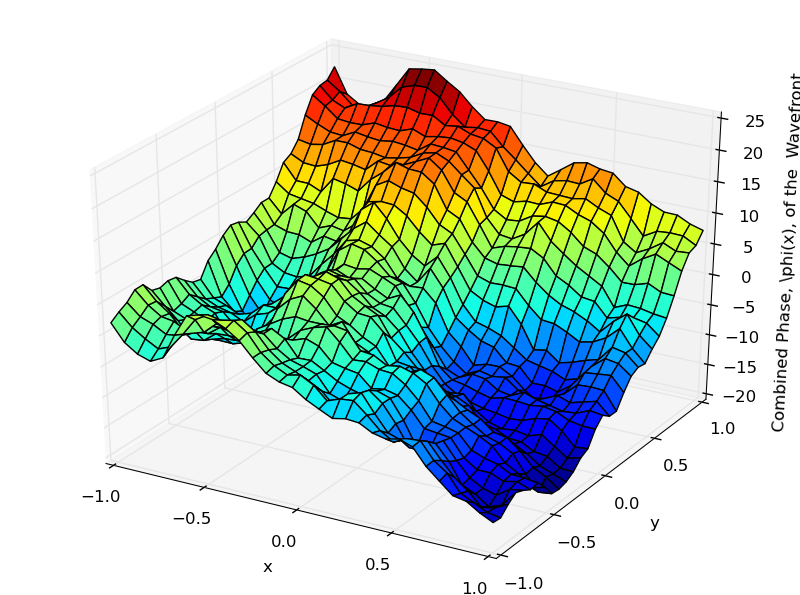
\includegraphics[height=0.5\textwidth, height=.3\textwidth]{Figures/kolmogorov.png}
	\caption{A realization of a Kolmogorov phase aberration, here with $r_0 = 0.1$, $p=3$ and $N_x,N_y = 30$.}
	\label{fig_wfg05}
\end{figure}

To conclude, Kolmogorov, von K{\'a}rm{\'a}n and Zernike are created in a similar manner. The final wavefront is simply a addition of both aberrations. This will not be discussed further.

\newpage
\section{WFG in Python}
This is a manual is intended as reference guide to show around the wavefront generation code of Adaptive Optics in Python. This manual will comprise of a description of the classes together with their methods and functions. A new page is made for every function, for readability, due to the many indentations, consider this when printing!

As of current, the WFG part includes two classes. One class on the Zernike aberrations. The second class is on the phase screens of the the wavefront, as for example Kolmogorov behaviour.

\lstset{language=Python} 
% Zernike static methods
\subsection{Zernike: Coding Example}
Coding Example: This code creates a wavefront consisting of three Zernike modes 2,4 and 21, with the corresponding weights 0.5, 0.25 and -0.6. The wavefornt is plotted and then decomposed. The array (vector) \texttt{a}, should return 0.5, 0.25 and -0.6! The computation \texttt{numpy.dot(numpy.transpose(z),z)} should return near identity as was described in the text earlier.

\texttt{zw = ZernikeWave()}

\texttt{zw.addMode([2,4,21], [.5,.25,-.6]) }

\texttt{W = zw.createWavefront(40,40)}

\texttt{zw.plotWavefront(40,40)}

\texttt{z,a = zw.decomposeWavefront(W)}

\newpage
\subsection{Zernike functions}
\subsubsection*{\texttt{Z = zernike(rho, theta,u,v = None)}}
\textbf{Arguments}
\begin{description}
\item[\texttt{rho}]\hfill \\
	Meshgrid array or scalar containing the distance from the optical origin $r$.
\item[\texttt{theta}]\hfill \\
 	Meshgrid array or scalar containing the cylindrical radial 	angle $\theta$. 
\item[\texttt{u}] \hfill \\
	$u$ mode index of the Zernike mapping, if $v$ is omitted, this is $i$ in Noll's mapping.
\item[\texttt{v}] \hfill \\
	 $v$ mode index of the Zernike mapping, this can be omitted if Noll's mapping is desired. 
\end{description}
\textbf{Returns}
\begin{description}
\item[\texttt{Z}] \hfill \\
 The $(u,v)$ or $i$ Zernike mode, on the grid points defined in \texttt{rho} and \texttt{theta}.
\end{description}

\newpage
\subsubsection*{\texttt{u,v = zernikeIndex(i)}}
\textbf{Arguments}
\begin{description}
\item[\texttt{i}] \hfill \\
Noll's mapping index
\end{description}
\textbf{Returns}
\begin{description}
\item[\texttt{u}] \hfill \\
$u$ of the Zernike mapping
\item[\texttt{v}] \hfill \\
$v$ of the Zernike mapping
\end{description}

\newpage
\subsection{ZernikeWave Class: Methods and Functions}
\subsubsection*{\texttt{zw = ZernikeWave()}}
\textbf{Arguments}
\begin{description}
	\item[\texttt{None}]
\end{description}
\textbf{Returns}
\begin{description}
	\item[\texttt{zw}]
	An instance of the ZernikeWave class
\end{description}

\newpage
\subsubsection*{\texttt{addMode(i, alpha\_i = 1)}}
\textbf{Arguments}
\begin{description}
  \item[\texttt{i}] \hfill \\
  Array or scalar containing the Zernike modes in Noll's mapping to add
  \item[\texttt{alpha\_i}] \hfill \\
  Array or scalar containing the weight of the modes specified, if omitted, a weight of one will be assumed. Ideal for decomposition, when the weighting is not important.
\end{description}
\textbf{Returns}
\begin{description}
	\item[\texttt{None}]
\end{description}

\newpage
\subsubsection*{\texttt{changeModeWeight(iModeToChange,alpha\_i = 1)}}
\textbf{Arguments}
\begin{description}
  \item[\texttt{i}] \hfill \\
  Array or scalar containing the Zernike modes in Noll's mapping to add
  \item[\texttt{alpha\_i}] \hfill \\
  Array or scalar containing the weight of the modes specified, if omitted, a weight of one will be assumed. Ideal for decomposition, when the weighting is not important.
\end{description}
\textbf{Returns}
\begin{description}
	\item[\texttt{None}]
\end{description}

\newpage
\subsubsection*{\texttt{removeMode(iToRemove)}}
\textbf{Arguments}
\begin{description}
  \item[\texttt{iToRemove}] \hfill \\
  Array or scalar containing the modes to remove.
\end{description}
\textbf{Returns}
\begin{description}
	\item[\texttt{None}]
\end{description}

\newpage
\subsubsection*{\texttt{exists = modeExists(i)}}
\textbf{Arguments}
\begin{description}
	\item[\texttt{i}]
	Scalar of Noll's index, to check.
\end{description}
\textbf{Returns}
\begin{description}
	\item[\texttt{exists}]
	Returns 1 (True) if mode is existent, else 0 (False).
\end{description}

\newpage
\subsubsection*{\texttt{i = getModes()}}
\textbf{Arguments}
\begin{description}
	\item[\texttt{None}]
\end{description}
\textbf{Returns}
\begin{description}
	\item[\texttt{i}]
	List or scalar, with the modes specified in this instance.
\end{description}

\newpage
\subsubsection*{\texttt{alpha\_i = getWeights()}}
\textbf{Arguments}
\begin{description}
	\item[\texttt{None}]
\end{description}
\textbf{Returns}
\begin{description}
	\item[\texttt{alpha\_i}]
	List or scalar, with the weights of the modes specified in this instance.
\end{description}

\newpage
\subsubsection*{\texttt{W = createWavefront(nX,nY)}}
\textbf{Arguments}
\begin{description}
  \item[\texttt{nX}] \hfill \\
  Number of elements in $x$-direction of the grid
  \item[\texttt{nY}] \hfill \\
 	Number of elements in $y$-direction of the grid
\end{description}
\textbf{Returns}
\begin{description}
	\item[\texttt{W}]
	The created wavefront, containing the zernike weights specified in the instance, on the grid elements specified, the spatial domain is in the unity circle.
\end{description}

\newpage
\subsubsection*{\texttt{Z,A = decomposeWavefront(W)}}
\textbf{Arguments}
\begin{description}
  \item[\texttt{W}] \hfill \\
  The wavefront to decompose
\end{description}
\textbf{Returns}
\begin{description}
	\item[\texttt{Z}]
	The constructed basis matrix $\mathcal{Z}$, can be used to check identity of $\mathcal{Z}^T \mathcal{Z}$ to determine the validity of the decomposition.
	\item[\texttt{A}]
	The computed weights, according to the weights sepified in the instance of the ZernikeWave class.
\end{description}

\newpage
\subsubsection*{\texttt{plotMode(iToPlot,nX,nY)}}
\textbf{Arguments}
\begin{description}
  \item[\texttt{iToPlot}]
  The mode in Noll's index to plot, can be used for checking intermediate results of the construction.
  \item[\texttt{nX}] \hfill \\
  Number of elements in $x$-direction of the grid
  \item[\texttt{nY}] \hfill \\
 	Number of elements in $y$-direction of the grid
\end{description}
\textbf{Returns}
\begin{description}
	\item[\texttt{None}]
\end{description}

\newpage
\subsubsection*{\texttt{plotWavefront(nX,nY)}}
\textbf{Arguments}
\begin{description}
  \item[\texttt{nX}] \hfill \\
  Number of elements in $x$-direction of the grid
  \item[\texttt{nY}] \hfill \\
 	Number of elements in $y$-direction of the grid
\end{description}
\textbf{Returns}
\begin{description}
	\item[\texttt{None}]
\end{description}

% Phasescreen dynamic class
\newpage
\subsection{PhaseScreen Class: Example}
Coding Example: Create a Kolmogorov phase screen with $r_0 = 0.1$. The other parameters $l_0$ and $L_0$ are specified but not used. They can be deleted. Also consider trying to replace 'Kolmogorov' by 'vonKarman' for a von K{\'a}rm{\'a}n pahse screen. The phase screen is then created and plotted.
\texttt{ps = PhaseScreen()}
\texttt{ps.setType('Kolmogorov') }
\texttt{ps.setParams(\{'r0' : .1, 'l0' : .01, 'L0' : 100\})}
\texttt{W = ps.createWavefront(40,40)}
\texttt{ps.plotWavefront(40,40)}

\newpage
\subsection{PhaseScreen Class: Methods and Functions}
\subsubsection*{\texttt{ps = PhaseScreen()}}
\textbf{Arguments}
\begin{description}
	\item[\texttt{None}]
\end{description}
\textbf{Returns}
\begin{description}
	\item[\texttt{ps}]
	An instance of the PhaseScreen class
\end{description}

\newpage
\subsubsection*{\texttt{setType(phaseScreenType = 'Kolmogorov'}}
\textbf{Arguments}
\begin{description}
	\item[\texttt{phaseScreenType}]
	A string containing the name of the phase screen to use, as of current, 'Kolmogorov' or 'vonKarman' can be used. If omitted, a Kolmogorov phase screen is assumed.
\end{description}
\textbf{Returns}
\begin{description}
	\item[\texttt{None}]
\end{description}

\newpage
\subsubsection*{\texttt{screenType = getType()}}
\textbf{Arguments}
\begin{description}
	\item[\texttt{None}]
\end{description}
\textbf{Returns}
\begin{description}
	\item[\texttt{screenType}]
	A string containing the name of the used phase screen.
\end{description}

\newpage
\subsubsection*{\texttt{setParams(parameters)}}
\textbf{Arguments}
\begin{description}
	\item[\texttt{screenType}]
	A 'dict' data type containing the the parameters of the phase screen. For Kolmogorov, 'r0' is used, for 'von Karman', 'r0', 'l0' and 'L0' is used. Use this format, as an example: \texttt{{'r0': 0.1, 'l0':0.1, 'L0' : 100}}. If more parameters are specified then necessary, the unused are omitted. If to few are specified the code throws an error.
\end{description}
\textbf{Returns}
\begin{description}
	\item[\texttt{None}]
\end{description}

\newpage
\subsubsection*{\texttt{params = getParameters()}}
\textbf{Arguments}
\begin{description}
	\item[\texttt{None}]
\end{description}
\textbf{Returns}
\begin{description}
	\item[\texttt{params}]
	A 'dict' datatype containing the parameters used by the specific type set-up. The returned format is similar to \texttt{setParameters(\dots)} and dependant on the set type: 'Kolmogorov' or 'von Karman'.
\end{description}

\newpage
\subsubsection*{\texttt{W = createWavefront(nX,nY)}}
\textbf{Arguments}
\begin{description}
  \item[\texttt{nX}] \hfill \\
  Number of elements in $x$-direction of the grid
  \item[\texttt{nY}] \hfill \\
 	Number of elements in $y$-direction of the grid
\end{description}
\textbf{Returns}
\begin{description}
	\item[\texttt{W}]
	The created wavefront, containing the set type screen specified in the instance, on the grid elements specified, the spatial domain is in the unity rectangle.
\end{description}

\newpage
\subsubsection*{\texttt{phi = kolmogorov(N, r0, D = 2.)}}
\textbf{Arguments}
\begin{description}
  \item[\texttt{N}] \hfill \\
  Number of elements in $x,y$-direction of the grid.
  \item[\texttt{r0}] \hfill \\
  The Fried parameter $r_0$, the caracteristic eddy or turbulent bubble size.
  \item[\texttt{D}] \hfill \\
 	The range on which to create the wavefront. By default, it is plotted on teh unity rechtangle, so the rectangle edge length D is 2, if anything else is desired, consider replacement.  
\end{description}
\textbf{Returns}
\begin{description}
	\item[\texttt{W}]
	The created wavefront, constructed via the subharmonics method, containing the set type screen specified in the instance, on the grid elements specified, the spatial domain is in the unity rectangle.
\end{description}

\newpage
\subsubsection*{\texttt{phi = vonkarman(N, r0, l0, L0, D = 2)}}
\textbf{Arguments}
\begin{description}
  \item[\texttt{N}] \hfill \\
  Number of elements in $x,y$-direction of the grid.
  \item[\texttt{r0}] \hfill \\
  The Fried parameter $r_0$, the caracteristic eddy or turbulent bubble size.
  \item[\texttt{l0}] \hfill \\
  The von Karman small length scale.
  \item[\texttt{L0}] \hfill \\
  The von Karman large length scale.
  \item[\texttt{D}] \hfill \\
 	The range on which to create the wavefront. By default, it is plotted on teh unity rechtangle, so the rectangle edge length D is 2, if anything else is desired, consider replacement. 
\end{description}
\textbf{Returns}
\begin{description}
	\item[\texttt{W}]
	The created wavefront, constructed via the subharmonics method, containing the set type screen specified in the instance, on the grid elements specified, the spatial domain is in the unity rectangle.
\end{description}

\newpage
\subsubsection*{\texttt{phi = hfkolmogorov(N, r0, D = 2.)}}
\textbf{Arguments}
\begin{description}
  \item[\texttt{N}] \hfill \\
  Number of elements in $x,y$-direction of the grid.
  \item[\texttt{r0}] \hfill \\
  The Fried parameter $r_0$, the caracteristic eddy or turbulent bubble size.
  \item[\texttt{D}] \hfill \\
 	The range on which to create the wavefront. By default, it is plotted on teh unity rechtangle, so the rectangle edge length D is 2, if anything else is desired, consider replacement.  
\end{description}
\textbf{Returns}
\begin{description}
	\item[\texttt{W}]
	The created wavefront, containing the set type screen specified in the instance, on the grid elements specified, the spatial domain is in the unity rectangle.
\end{description}

\newpage
\subsubsection*{\texttt{phi = hfvonkarman(N, r0, l0, L0, D = 2)}}
\textbf{Arguments}
\begin{description}
  \item[\texttt{N}] \hfill \\
  Number of elements in $x,y$-direction of the grid.
  \item[\texttt{r0}] \hfill \\
  The Fried parameter $r_0$, the caracteristic eddy or turbulent bubble size.
  \item[\texttt{l0}] \hfill \\
  The von Karman small length scale.
  \item[\texttt{L0}] \hfill \\
  The von Karman large length scale.
  \item[\texttt{D}] \hfill \\
 	The range on which to create the wavefront. By default, it is plotted on teh unity rechtangle, so the rectangle edge length D is 2, if anything else is desired, consider replacement. 
\end{description}
\textbf{Returns}
\begin{description}
	\item[\texttt{W}]
	The created wavefront, containing the set type screen specified in the instance, on the grid elements specified, the spatial domain is in the unity rectangle.
\end{description}

\newpage
\subsubsection*{\texttt{W = plotWavefront(nX,nY)}}
\textbf{Arguments}
\begin{description}
  \item[\texttt{nX}] \hfill \\
  Number of elements in $x$-direction of the grid
  \item[\texttt{nY}] \hfill \\
 	Number of elements in $y$-direction of the grid
\end{description}
\textbf{Returns}
\begin{description}
	\item[\texttt{None}]
\end{description}

\newpage
\subsection{Support Functions}
The following functions are used inside the phase screen and zernike classes to provide some services that show up more often.

\subsubsection*{\texttt{f = kroneckerDelta(x)}}
\textbf{Arguments}
\begin{description}
	\item[\texttt{x}]
	The input argument.
\end{description}
\textbf{Returns}
\begin{description}
	\item[\texttt{f}]
	Dirac delta function, $\infty$ on $x=0$, zero otherwise.
\end{description}

\newpage
\subsubsection*{\texttt{f = gamma2(n)}}
\textbf{Arguments}
\begin{description}
	\item[\texttt{x}]
	The input argument.
\end{description}
\textbf{Returns}
\begin{description}
	\item[\texttt{f}]
	Factorial or gamma function, $\infty$ for $x<0$, else it returns the factorial. Recall: Gamma$(n+1) = n!$, currently a lazy implementation, without the need to add 1 to the argument. The function does NOT solve $int_{0}^{inf} = t^{n-1}*e^{-t} dt$. It only extends validity beyond $n < 0$. The result is only guaranteed for integer arguments.
\end{description}

\newpage
\subsubsection*{\texttt{R,Theta = cart2pol(X,Y)}}
\textbf{Arguments}
\begin{description}
	\item[\texttt{X}]
	The position on the x axis in meshgrid format.
	\item[\texttt{X}]
	The position on the y axis in meshgrid format.
\end{description}
\textbf{Returns}
\begin{description}
	\item[\texttt{R}]
	The position on the $r$ axis in meshgrid format.
	\item[\texttt{Theta}]
	The position on the $\theta$ axis in meshgrid format.
\end{description}

\newpage
\subsubsection*{\texttt{X,Y = pol2cart(R,Theta}}
\textbf{Arguments}
\begin{description}
	\item[\texttt{R}]
	The position on the $r$ axis in meshgrid format.
	\item[\texttt{Theta}]
	The position on the $\theta$ axis in meshgrid format.
\end{description}
\textbf{Returns}
\begin{description}
	\item[\texttt{X}]
	The position on the x axis in meshgrid format.
	\item[\texttt{X}]
	The position on the y axis in meshgrid format.
\end{description}

\newpage
\subsubsection*{\texttt{X,Y = createGrid(nX, nY,rangeX=[-1,1],rangeY=[-1,1])}}
\textbf{Arguments}
\begin{description}
	\item[\texttt{nX}]
	Distance between grid point on the x-axis.
	\item[\texttt{nY}]
	Distance between grid point on the y-axis.
	\item[\texttt{rangeX}]
	The x range where the grid is defined, assumes a unity rectangle by default.
	\item[\texttt{rangeY}]
	The y range where the grid is defined, assumes a unity rectangle by default.
\end{description}
\textbf{Returns}
\begin{description}
	\item[\texttt{f}]
	Returns a meshgrid, with a specified number of elements in both x an y direction. Additionally, the range can be specified, if the ranges are not specified, it is assumed to be in [-1,1] 
\end{description}

\newpage
\subsubsection*{\texttt{inCircle = circ(X,Y,radius = 1.,datatype = 'bool')}}
\textbf{Arguments}
\begin{description}
	\item[\texttt{X}]
	The position on the x axis in meshgrid format.
	\item[\texttt{X}]
	The position on the y axis in meshgrid format.
	\item[\texttt{radius}]
	The radius to define the aperture radius with. Set to one by default.
	\item[\texttt{datatype}]
	The datatype to return. Set to boolean by default.
\end{description}
\textbf{Returns}
\begin{description}
	\item[\texttt{f}]
	Returns a circular aperture based on the grid X and Y in the specified datatype. The radius is assumed at one, if it is not specified. Whether to include the boundary of the circle can be a topic of discussion.
\end{description}

\newpage
\section{Appendix: Maxwell Equations}
\subsection{Obtaining the Wave-Equation}
Maxwell equations provide insight of the behaviour of light a continues wave, that propagates through a medium. In the case of a homogeneous, non-dispersive medium in absence of charges, Maxwell's equations reduce to a neat wave equation.

To get to the wave description of the Maxwell equations, start with the orthogonality between the electric field and the magnetic field, as decribed by  Faraday's law. First take the curl of Faraday's law, by multiplying it with the gradient operator in \ref{eq_wfga1} on both sides. The electric field is described by the vector $E$, the magnetic field is represented by $B$. Both $\mu$ and $\epsilon$ are material dependant constants.
\begin{equation}
\label{eq_wfga1}
\nabla \times (\nabla \times E) = -\frac{\partial}{\partial t}(\nabla \times B)
\end{equation}

Now consider Amp\`{e}re's law below in equation \ref{eq_wfga2}.
\begin{equation}
\label{eq_wfga2}
\nabla \times B = \mu \left( J + \epsilon \frac{\partial E}{\partial t} \right)
\end{equation}

Then substitute Amp\`{e}re's law in Faraday's law. Further, since no charge was assumed, the charge density $J$ can be set to zero, as below in \ref{eq_wfga3}.
\begin{equation}
\label{eq_wfga3}
\nabla \times (\nabla \times E) = -\mu \epsilon \frac{\partial^2}{\partial t^2} E
\end{equation}

Now consider the vector identity from equation \ref{eq_wfga4}.
\begin{equation}
\label{eq_wfga4}
\nabla \times (\nabla \times E) = \nabla(\nabla \cdot E) - \nabla^2 E
\end{equation}

The reason for introducing the identity in equation \ref{eq_wfga4} becomes obvious when considering Gauss' law below in equation \ref{eq_wfga5}. Now note that the gradient of the scalar $\nabla \cdot E$ is zero.
\begin{equation}
\label{eq_wfga5}
\nabla \cdot E = \frac{\rho}{\epsilon}
\end{equation}

Thus reducing to equation \ref{eq_wfga6} below. It is now apparent that the equation is second order time dependant differential equation.
\begin{equation}
\label{eq_wfga6}
\nabla^2 E - \mu \epsilon \frac{\partial^2}{\partial t^2} E = 0 
\end{equation}

Similar manipulations can also be done for the magnetic field, start here with taking the curl of Amp\`{e}re's law and substituting Faraday's law into it. The wave equation for the magnetic field is described in equation \ref{eq_wfga7}.
\begin{equation}
\label{eq_wfga7}
\nabla^2 B - \mu \epsilon \frac{\partial^2}{\partial t^2} B = 0 
\end{equation}

For Cartesian coordinates, the Laplacians $\nabla^2 E$ and $\nabla^2 B$ are i independent with respect to the coordinates. Giving rise to equation with the intensity vector $U(r,t)$ in equation \ref{eq_wfga8}
\begin{equation}
\label{eq_wfga8}
\left( \nabla^2 - \mu \epsilon \frac{\partial^2}{\partial t^2} \right) U(r,t)= 0 
\end{equation}

The common way to solve these second order time dependant wave equations, is by separating the it into a spatial part and a time dependant part. Giving the result as is in equation \ref{eq_wfga9}. Note now the constant $\mu \epsilon$ can the repalced by the wave number $k = 2\pi/\lambda $ an the wave propagation speed $c = 1/\sqrt{\mu_0 \epsilon_0}$.
\begin{equation}
\label{eq_wfga9}
\end{equation}

\newpage
\bibliography{refs}
\bibliographystyle{ieeetran}
\end{document}

